\documentclass[11pt]{article}
\usepackage[T1]{fontenc}
\usepackage{lmodern}
\usepackage{parskip}
\usepackage[colorlinks=true,urlcolor=Blue,linkcolor=black,citecolor=black]{hyperref}
\usepackage{graphicx}
\usepackage{amsmath}
\usepackage[utf8]{inputenc}
\usepackage[spanish]{babel}
\usepackage{fancyhdr}
\usepackage{csquotes}
\usepackage{lastpage}
\usepackage{array}
\usepackage{listings}
\usepackage{color}
\definecolor{dkgreen}{rgb}{0,0.6,0}
\definecolor{gray}{rgb}{0.5,0.5,0.5}
\definecolor{mauve}{rgb}{0.58,0,0.82}
\usepackage[affil-it]{authblk}
\usepackage[activate={true,nocompatibility},final,tracking=true,kerning=true,spacing=true,factor=1100,stretch=10,shrink=10]{microtype}
\usepackage[hmargin=2cm,top=4cm,headheight=65pt,footskip=65pt]{geometry}
\usepackage{hyperref}
\usepackage{graphicx}
\graphicspath{ {./screenshots/p02/} }

% Documento
\begin{document}
% Título
\title{IFA. Práctica de laboratorio 02}
\author{Hugo Fonseca Díaz \\ email \href{mailto:uo258318@uniovi.es}{uo258318@uniovi.es}}
\affil{Escuela de Ingeniería Informática. Universidad de Oviedo.}
\maketitle
% Ejercicio 1
\section{Ejercicio 1}
Se guarda la fecha y hora del sistema en el archivo \verb|ej01.txt| con el comando \verb|date > ej01.txt|. Se muestra ese archivo con el comando \verb|cat|.
\begin{figure}[h!]
  \caption{Ejercicio 1: Resultado del comando \textit{cat ej01.txt}.}
  \centering
  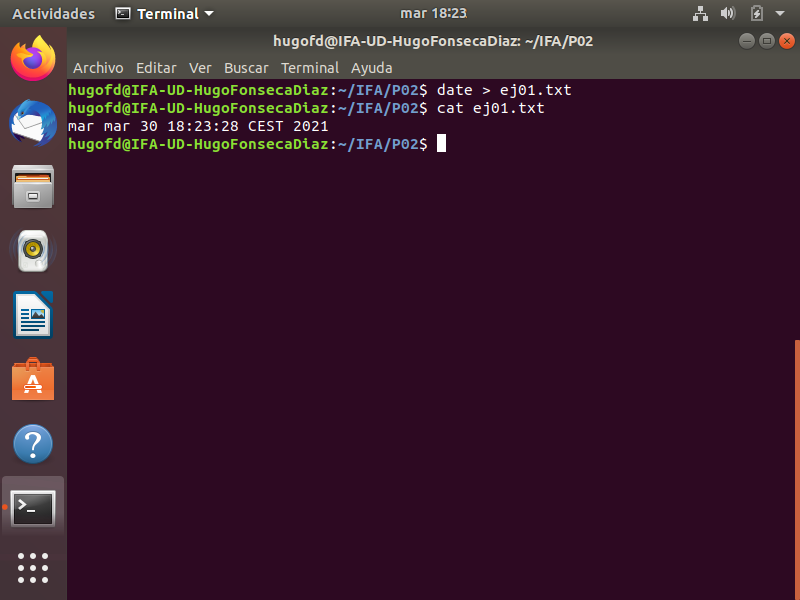
\includegraphics{e1-1.png}
\end{figure}

Se accede al sitio web \url{https://time.is/es/Spain} y se comprueba que la hora es la misma.
\begin{figure}[h!]
    \caption{Ejercicio 1: Hora en el sitio web \textit{time.is}.}
  \centering
  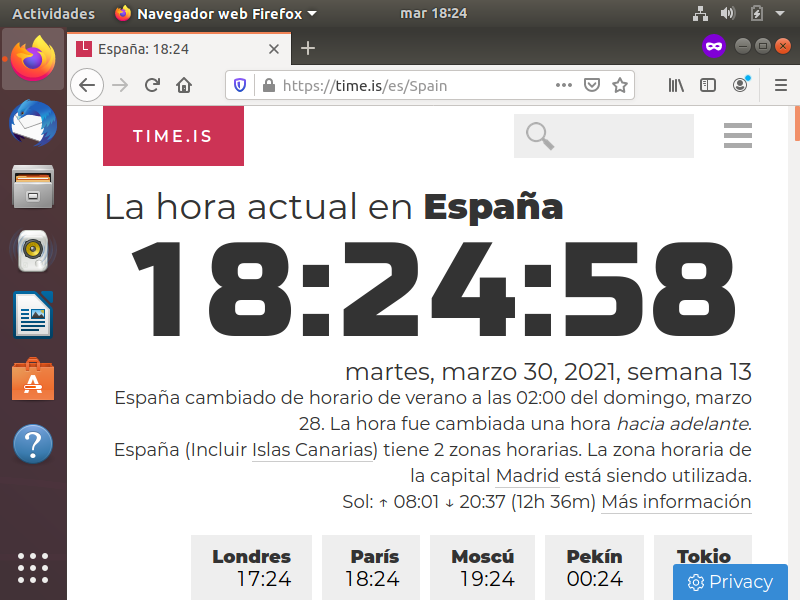
\includegraphics{e1-2.png}
\end{figure}
% Ejercicio 2
\section{Ejercicio 2}
Se utiliza el comando \verb|uname| con las opciones \verb|v| (lista la versión del kernel) y \verb|o| (lista el nombre del sistema operativo).
\begin{figure}[h!]
    \caption{Ejercicio 2: \textit{uname -vo}.}
  \centering
  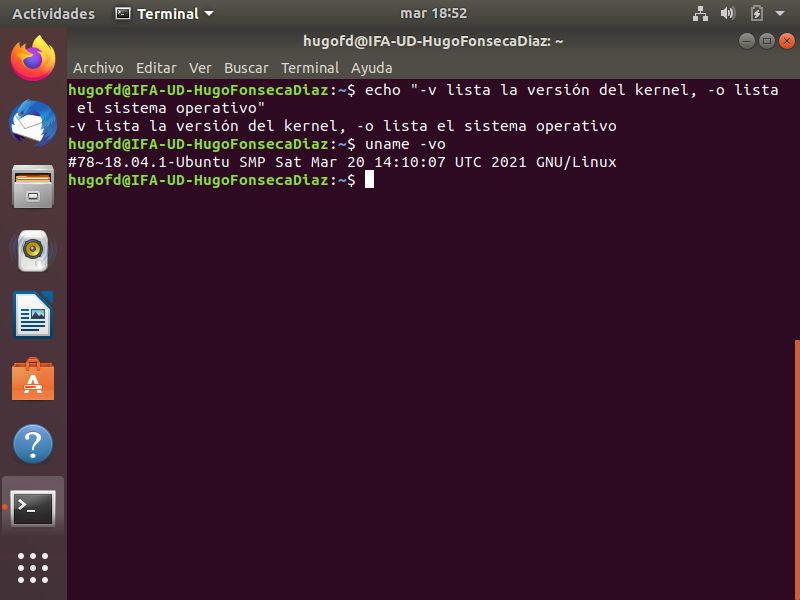
\includegraphics{e2.png}
\end{figure}
% Ejercicio 3
\section{Ejercicio 3}
Se utiliza el comando \verb|lshw|, primero con la flag \verb|short| para encontrar el nombre de la clase de los dispositivos de red.
\begin{figure}[h!]
    \caption{Ejercicio 3: \textit{lshw -short}.}
  \centering
  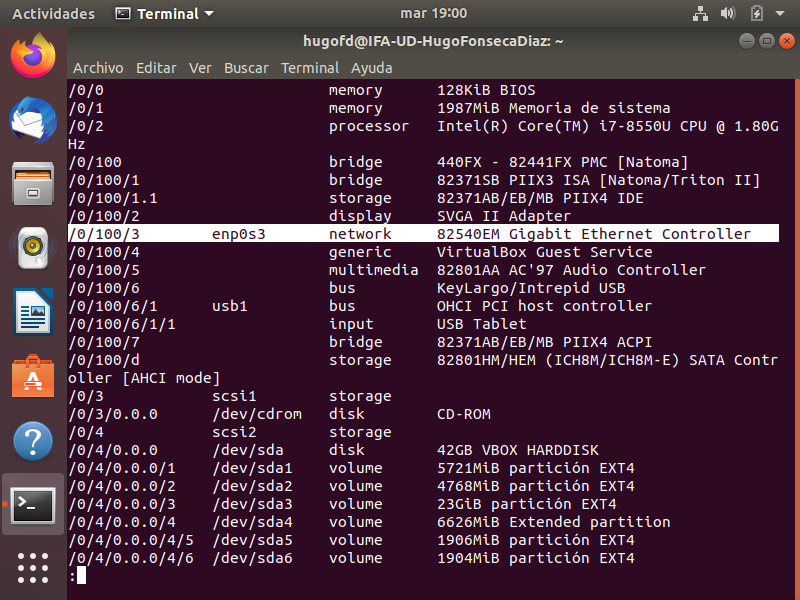
\includegraphics{e3-1.png}
\end{figure}

Una vez se sabe que el nombre de la clase de los dispositivos de red es \verb|network|, se utiliza el comando \verb|lshw| con la flag \verb|-class network|.
\begin{figure}[h!]
    \caption{Ejercicio 3: \textit{lshw -class network}.}
  \centering
  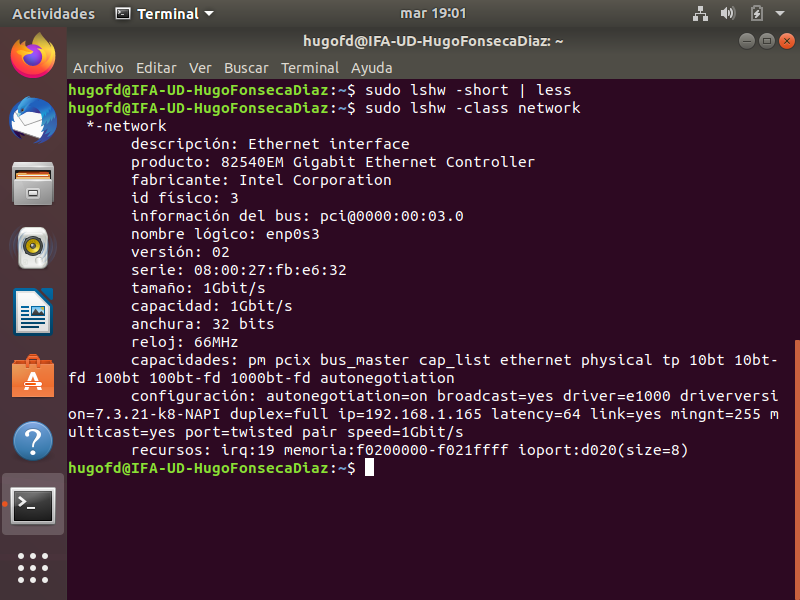
\includegraphics{e3-2.png}
\end{figure}
% Bibliografía
\begin{thebibliography}{8}
\end{thebibliography}
\end{document}


